\documentclass[12pt,a3paper]{article}
\usepackage{better_poster}


% ---- fill in from here

% authors
\title{A walking bipedal robot}
\author{A project in IN5590 by Lazo Omar E-mail: lazoo@ifi.uio.no }

% type of poster: [exp]erimental results, [methods], [theory]
% Disclaimer: the original classification had "study" and "intervention" as separate categories. I group them under experimental results.
\newcommand\postertype{exp} % [exp],[methods],[theory]

\begin{document}

% main point of your study
\makefinding{
\textbf{Lil Runner}
}


% \makemain{
% }{

% }


% the main text of your poster goes here
\makemain{
    % you can have 1 or 2 columns
    \raggedcolumns
    \begin{multicols}{2}
        \section{Intro}
        The project is a culmination of my efforts in the IN5590 course. The objective was to create a bipedal walking robot utilizing servos. This endeavor challenged my skills in CAD design, manufacturing, and programming. Ultimately, I was able to finalize the robot's design and bring it to life.
        
        \vspace{10}
        
        The primary goals for this project were:
        \begin{itemize}
            \setlength\itemsep{0.1em}
            \item Ensure that Lil Runner lives up to its name by achieving high-speed locomotion.
            \item Design Lil Runner to have an appealing and intriguing appearance.
        \end{itemize}
    
        Early design concepts and the final iteration of Lil Runner are featured in the \textbf{Extra figures} section.
    
        \section*{Tools}
        Key components used in this project include:
        \begin{itemize}
            \setlength\itemsep{0.1em}
            \item 6 Dynamixel AX12 servos
        \end{itemize}
    
        \vspace{10}
    
        The software tools that were essential for this project are:
        \begin{itemize}
            \setlength\itemsep{0.1em}
            \item SolidWorks (for CAD design)
            \item Cura (for 3D printing)
            \item Python (as the programming language)
            \item dynamixel\_sdk (a package for controlling the Dynamixel servos)
        \end{itemize}
    
        \columnbreak
    
        \section*{Conclusion}
        Lil Runner successfully achieved a notable and interesting design while being capable of a quick walking motion, described as more of a march rather than a jog. Given the time constraints, I was unable to achieve actual running movement.
    
        \vspace{10}
    
        Throughout this project, I tuned a sine controller for the servos to maximize Lil Runner's walking speed. Future enhancements could include employing AI algorithms, such as evolutionary algorithms or reinforcement learning, to optimize movement patterns further. Additionally, aesthetic improvements like adding lenses to Lil Runner's eyes, integrating lights, or applying a paint job could enhance its overall appearance, making it even more striking and engaging.
    
    
    \end{multicols}
}
% If you have extra figures or data to show
\makeextracolumn{

    \textit{Concept art of Lil Runner}
    
    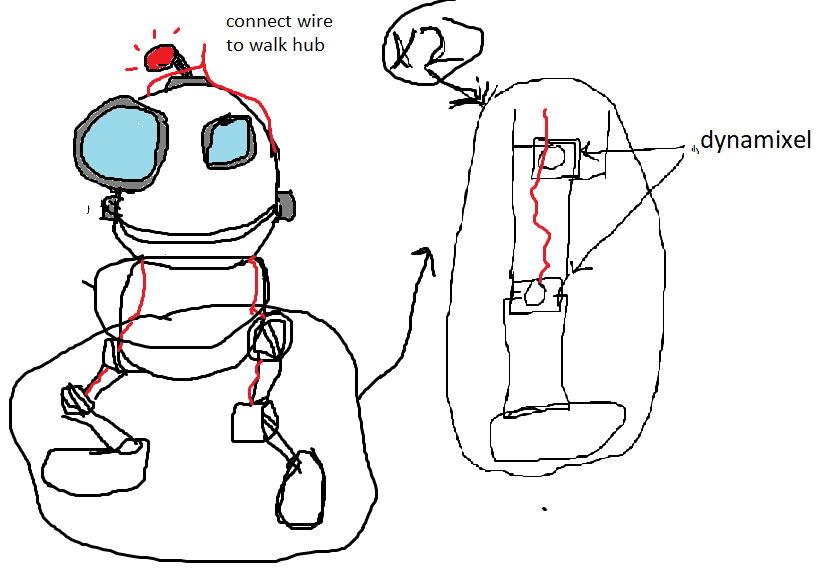
\includegraphics[width=1\linewidth]{concept_art.png}

    \textit{CAD design of Lil Runner}

    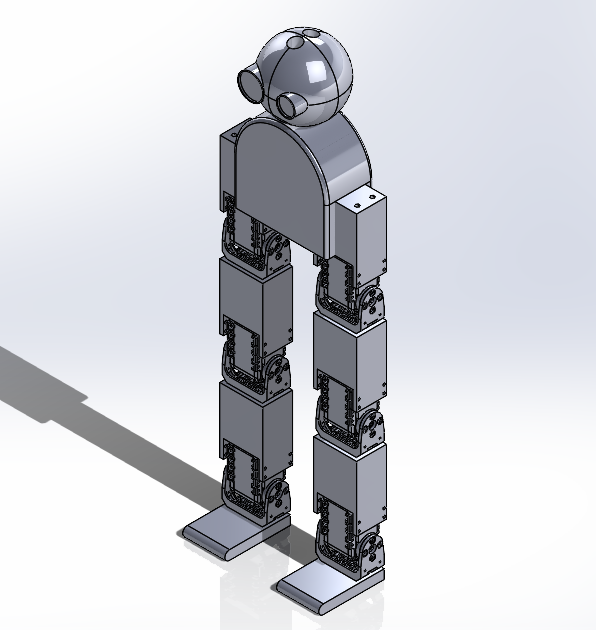
\includegraphics[width=1\linewidth, height=.8\linewidth]{images/1assembled.PNG}

    \textit{A picture of Lil Runner in the middle of marching}  
    
    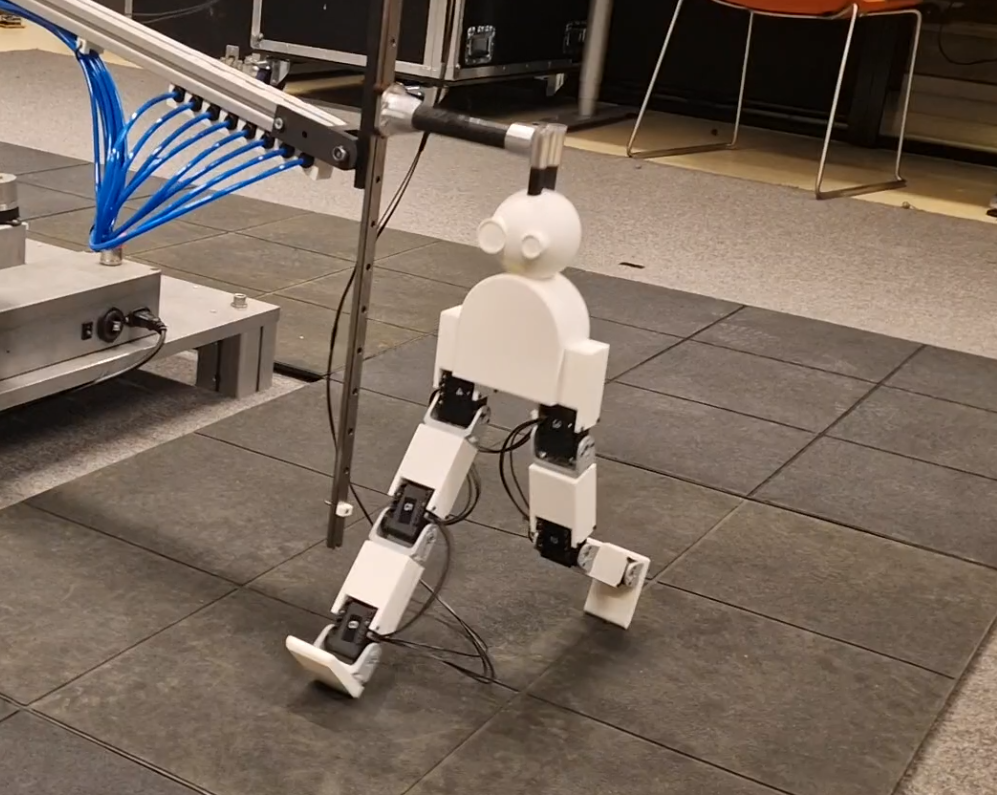
\includegraphics[width=1\linewidth]{2.png}
    
}

% footer
% generate qr code from https://www.qr-code-generator.com/ and replace qr_code.png
% default: barcode on the left
\makealtfooter{images/uni_logo.pdf}{images/qr-code.png}

% replace with this like for barcode on the right
%\makealtfooter{images/uni_logo.png}{images/qr-code.png}
 
\end{document}
